\hypertarget{a00842}{}\section{Troubleshooting}
\label{a00842}\index{Troubleshooting@{Troubleshooting}}
How to solve common issues. 

\hypertarget{a00842_troubleshooting_contents}{}\subsection{Contents}\label{a00842_troubleshooting_contents}
\begin{DoxyItemize}
\item \mbox{\hyperlink{a00842_troubleshooting_signature}{Plug-\/\+In Fails to Load in Shipping Pro Tools}}\end{DoxyItemize}
\hypertarget{a00842_troubleshooting_signature}{}\subsection{Plug-\/\+In Fails to Load in Shipping Pro Tools}\label{a00842_troubleshooting_signature}
If your plug-\/in fails to load in shipping Pro Tools with the message \char`\"{}\+The following plug-\/ins failed to load because they are not valid 64 bit A\+A\+X plug-\/ins\char`\"{} then the most likely reason is that the plug-\/in does not have a valid digital signature.

Your A\+AX plug-\/ins will not be compatible with shipping versions of Pro Tools until they are digitally signed using tools provided by P\+A\+CE Anti-\/\+Piracy, Inc. As an A\+AX developer you can receive these tools free of charge. Read the \mbox{\hyperlink{a00830_subsection__digital_signature_}{Digital signature}} section of the \mbox{\hyperlink{a00830}{Pro Tools Guide}} to learn about the digital signing requirements for compatibility with Pro Tools.

 

To verify whether this failure is due to an invalid digital signature vs. some other library loading failure, check the Pro Tools \mbox{\hyperlink{a00834}{log file}}. A failure caused by an invalid digital signature will result in log lines like the following\+:

\begin{DoxyVerb}Sys_PACE::GetDigitalSignature - looking for Eden dsig for path "/Applications/ProTools/Plug-Ins/DemoGain_example.aaxplugin/"
Sys_PACE::GetDigitalSignature - dsig error name /Applications/ProTools/Plug-Ins/DemoGain_example.aaxplugin/ 0 
legacy Dsig check disabled??
Sys_PACE::GetDigitalSignature - did NOT get valid dsig /Applications/ProTools/Plug-Ins/DemoGain_example.aaxplugin/
Plug-In Binary "DemoGain_example.aaxplugin" failed to load with err = -7054.
Plug-In Binary "DemoGain_example.aaxplugin" 1.0 : Failed to load.\end{DoxyVerb}


Another way to check whether a plug-\/in\textquotesingle{}s digital signature is invalid is to test the plug-\/in in a Pro Tools developer build or with the \mbox{\hyperlink{a00835}{Digi\+Shell}} utility. If the plug-\/in successfully loads and runs in these tools but not in a shipping build of Pro Tools then it is very likely that the problem is in the plug-\/in\textquotesingle{}s digital signature.

If you are having an issue running the signing tools then please check this list of the most common failure points\+:


\begin{DoxyEnumerate}
\item Bad command line arguments for {\ttfamily wraptool}  
\item An invalid developer certificate  
\item An expired developer certificate  
\item The Eden Tools license is not activated to your i\+Lok U\+SB key  
\item Your code signing certificate is not installed on your i\+Lok U\+SB key  
\item For Mac, the Xcode command line tools are not installed on your signing system  
\item The plug-\/in bundle itself is malformed and will not load  
\item The plug-\/in bundle is being modified at some point after being signed, thereby invalidating its digital signature  
\end{DoxyEnumerate}

If a digital signature was successfully applied to an A\+AX plug-\/in at one point in the build process but now the plug-\/in fails to load due to a bad signature then the most likely reason is that someone or something has tampered the signature or the .aaxplugin bundle thereby invalidating the signature.

Several things can cause this, for example symlinks not being preserved when copying the plug-\/in, an actual tampering of the plug-\/in, or corruption of the plug-\/in binary to name a few. Note that the A\+AX digital signature covers the entire .aaxplugin bundle so any actions which affect the contents of this bundle in any way after signing will invalidate the bundle\textquotesingle{}s digital signature.

If the failure is occurring on an isolated system then replacing the .aaxplugin which has an invalidated signature with an original, untampered copy (e.\+g. via a reinstall) should resolve this issue. Collaboration diagram for Troubleshooting\+:
\nopagebreak
\begin{figure}[H]
\begin{center}
\leavevmode
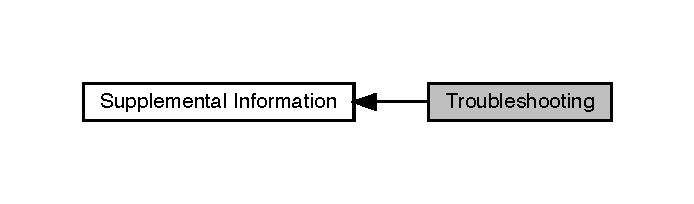
\includegraphics[width=333pt]{a00842}
\end{center}
\end{figure}
